\appendix
\section{备份}

\begin{frame}[label=appendix-1]{A1 · 主题时间与覆盖率}
  \crumb{备份}{主题完整分布}{Table 3 · p.\,48}
  \centering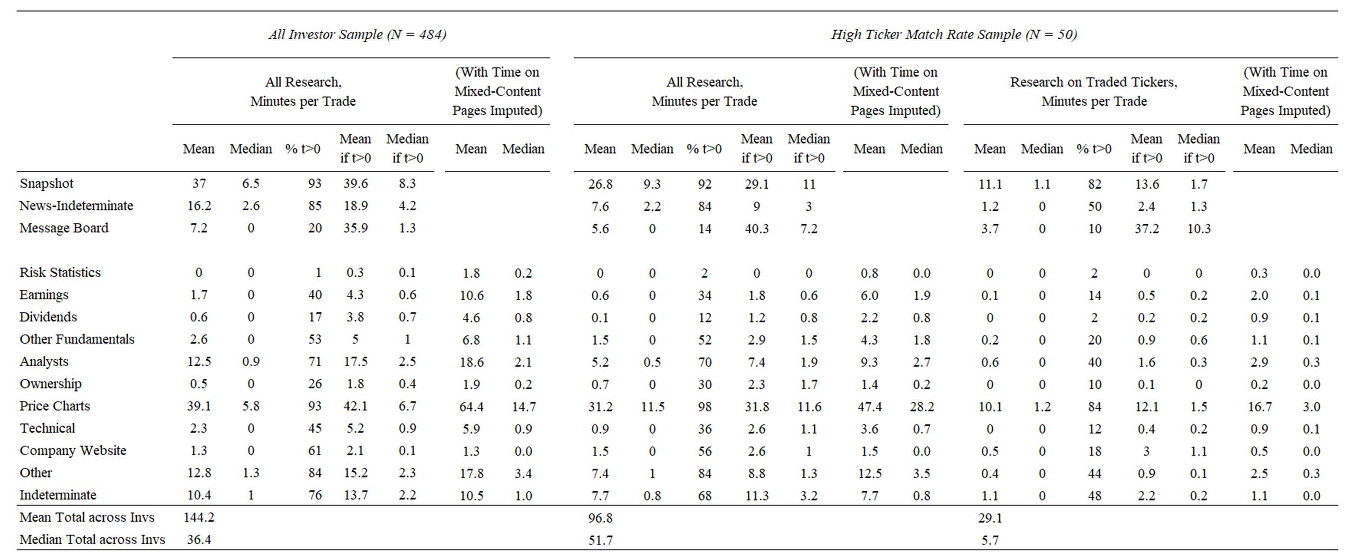
\includegraphics[width=\linewidth,height=5.2cm,keepaspectratio]{table3.pdf}\par
  \small 三块分别为 484 户全部股、50 户全部股、50 户交易标的。每块先读直接分类，再读插补。
  \par\smallskip\jump{topics}{返回 · 主题图}
\end{frame}

\begin{frame}[label=appendix-2]{A2 · 股票月回归的六列估计}
  \crumb{备份}{Table 4 上下两页}{pp.\,49--50}
  \pair{\centering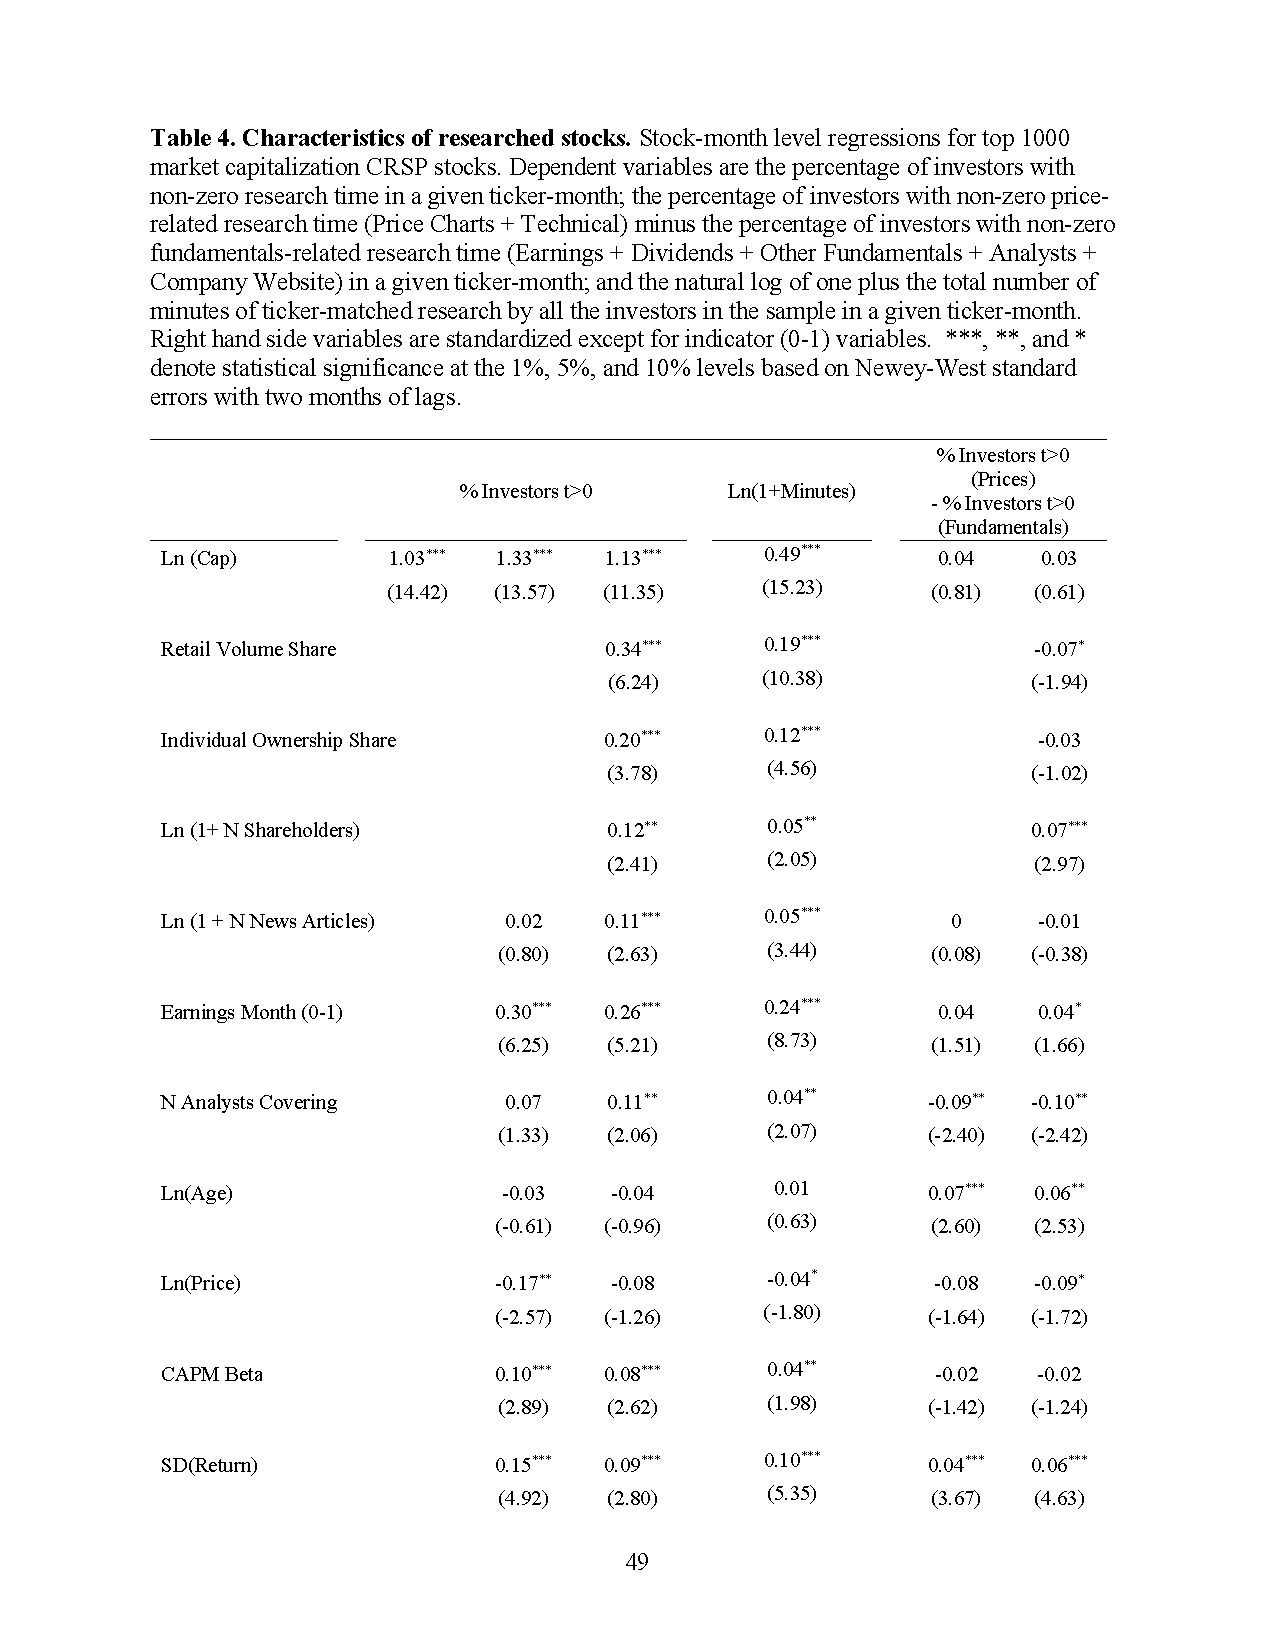
\includegraphics[width=\linewidth,height=4.9cm,keepaspectratio,trim=55bp 75bp 55bp 70bp,clip]{table4-p49.pdf}\par}
       {\centering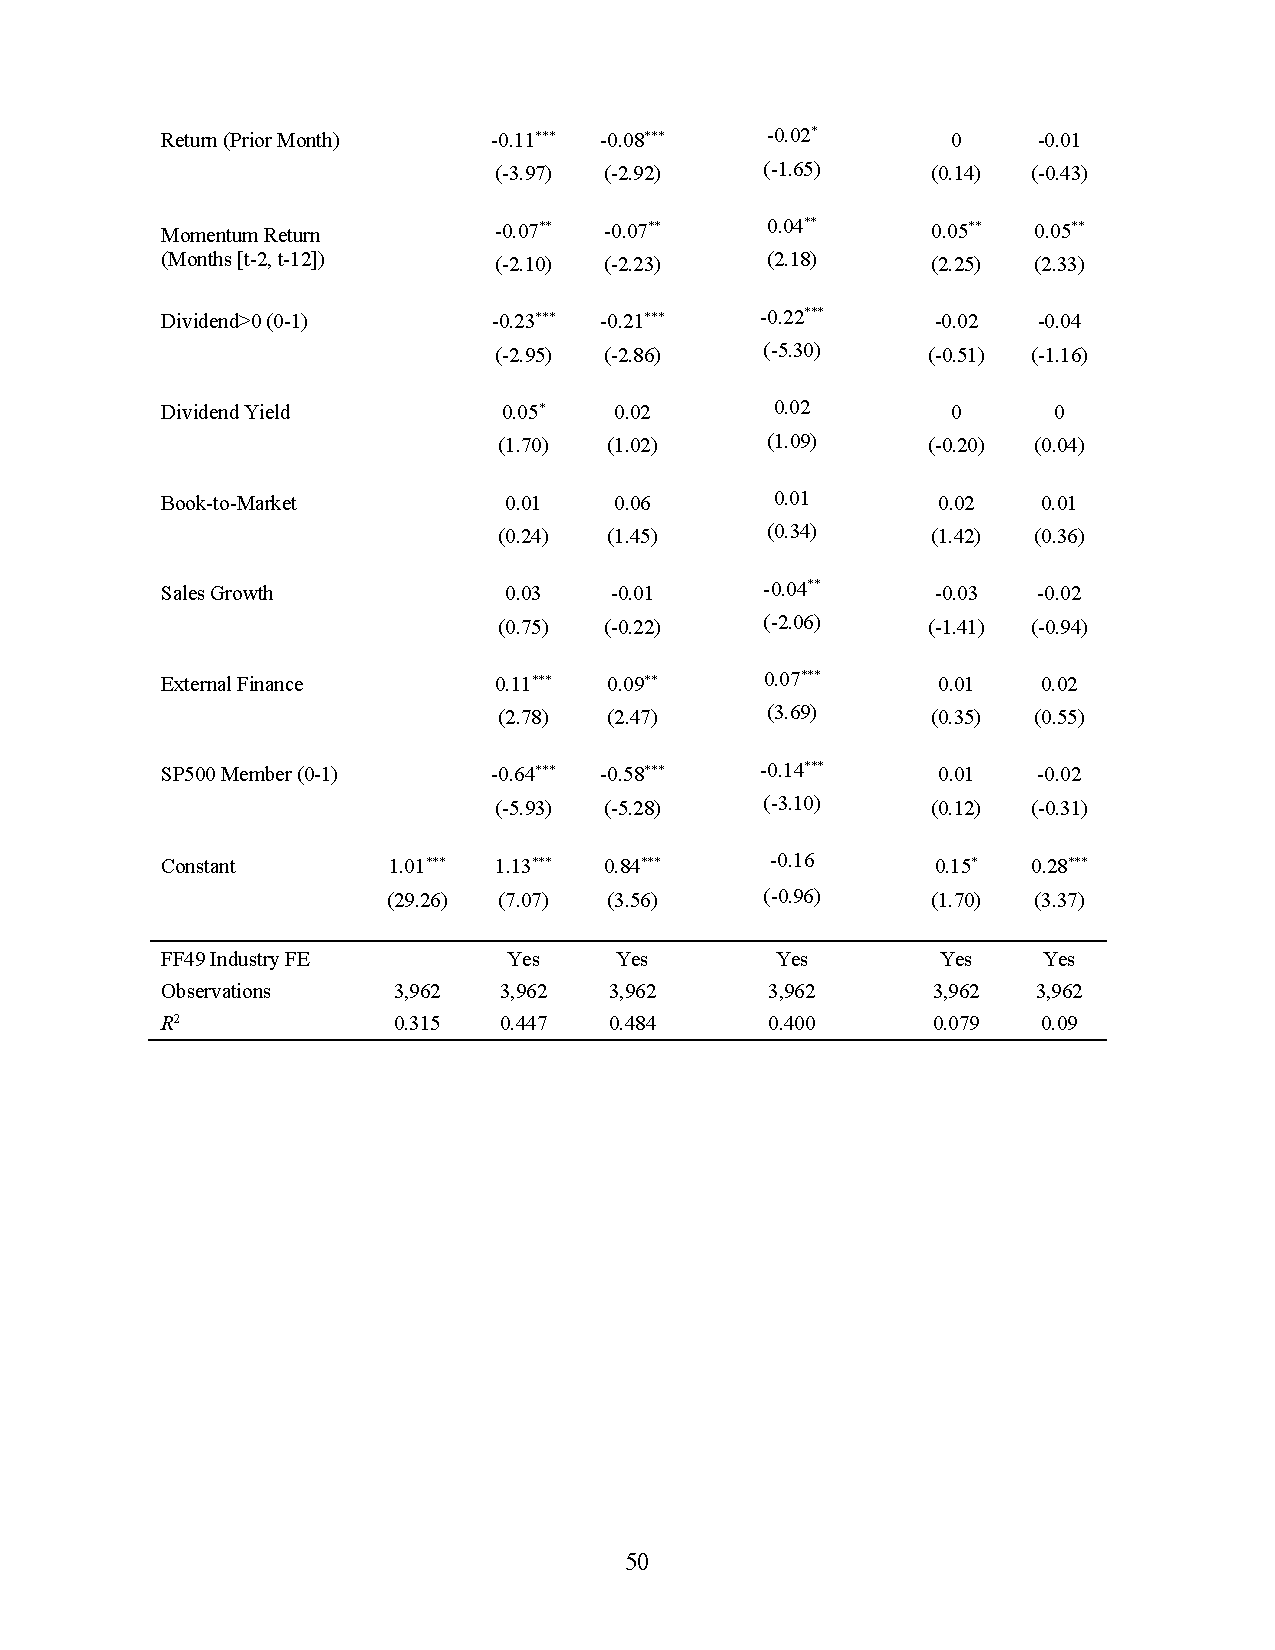
\includegraphics[width=\linewidth,height=4.9cm,keepaspectratio,trim=55bp 95bp 55bp 75bp,clip]{table4-p50.pdf}\par}
  \small (1)--(3) 覆盖率，(4) 对数总分钟，(5)--(6) 内容倾斜。\par
  \jump{design}{返回 · 规格与因变量}
\end{frame}

\begin{frame}[label=appendix-3]{A3 · 混合页的三种权重}
  \crumb{备份}{插补口径}{Table IA2 · p.\,70}
  \small
  \renewcommand{\arraystretch}{1.08}
  \begin{tabularx}{\linewidth}{@{}L{.21\linewidth}YY@{}}\toprule
  内容来源 & 权重设计 & 价格图所占比例\\\midrule
  快照 · 等权 & 在该页面可辨认类别之间平分 & 10\%–33\%（跨域名）\\
  快照 · 视觉 & 按页面上各内容占据的行数分配 & 38\%–79\%（跨域名）\\
  快照 · 兴趣 & 按各类专门页面的主动研究比例分配 & 18\%–49\%（跨域名）\\
  留言板 & 用当代 Reddit 帖子主题估计 & 26\%\\
  未确定新闻 & 用部分券商的标题配对 RavenPack & 12\%\\\bottomrule
  \end{tabularx}
  正文用兴趣权重，区间为跨域名范围。\par
  \jump{mixed}{返回 · 混合页归因}
\end{frame}

\begin{frame}[label=appendix-4]{A4 · 点击数据的十步处理}
  \crumb{备份}{原文 Internet Appendix}{pp.\,58--68}
  \small
  \begin{tabularx}{\linewidth}{@{}rY rY@{}}
    \toprule 步 & 处理 & 步 & 处理\\\midrule
    1 & 读取券商订单、匹配证券、合并重复 & 6 & 区分其他券商浏览、研究和交易\\
    2 & 统一链接编码与域名、划会话 & 7 & 甄别公司官网并限制用时\\
    3 & 对照历史页面、读代码与主题 & 8 & 用相邻同股研究补配缺码链接\\
    4 & 拆多标的／复合图表 & 9 & 归到 11 类以及三种混合格式\\
    5 & 统一股票代码、匹配 CRSP & 10 & 将混合页时间插补到主题\\\bottomrule
  \end{tabularx}\par\medskip
  \jump{rules}{返回 · 三条上屏规则}
\end{frame}

\begin{frame}[label=appendix-5]{A5 · 画像与研究用时的原表}
  \crumb{备份}{样本和分位数}{Tables 1--2 · pp.\,46--47}
  \pair{\centering\small\textbf{Table 1 · 投资者画像}\par
    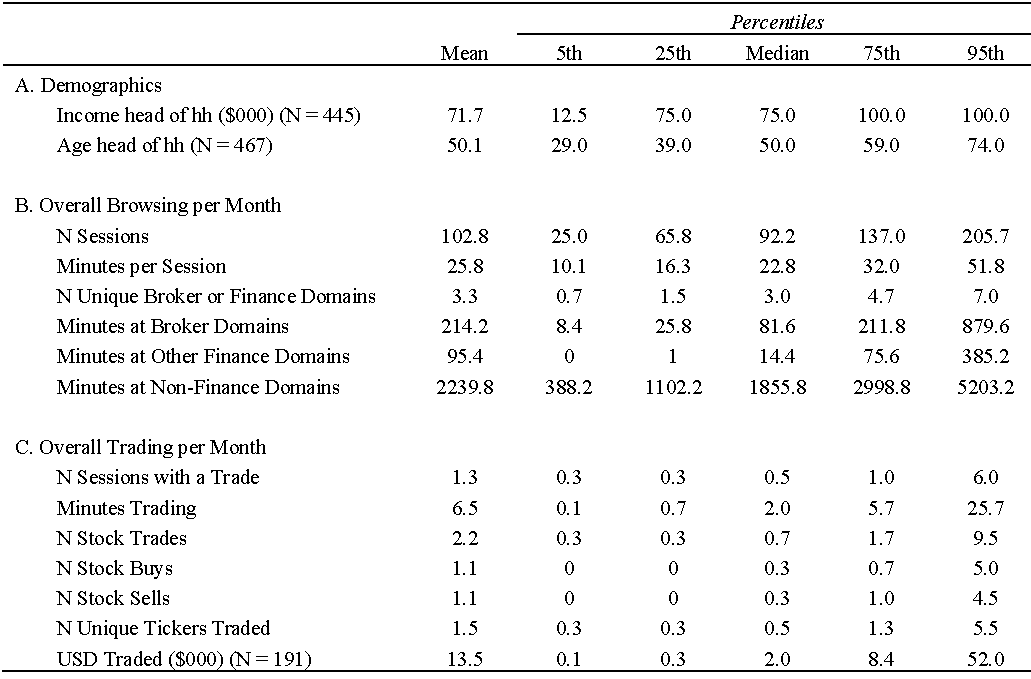
\includegraphics[width=\linewidth,height=5.2cm,keepaspectratio]{table1.pdf}\par}
  {\centering\small\textbf{Table 2 · 研究活动}\par
    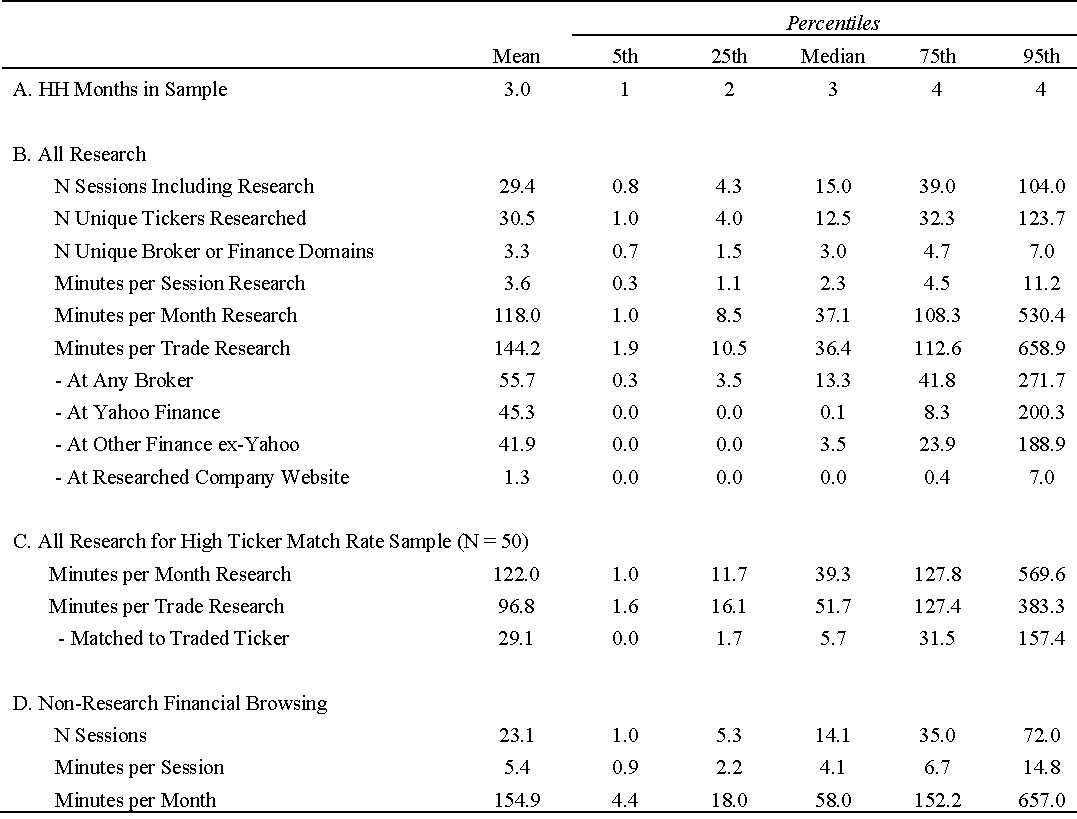
\includegraphics[width=\linewidth,height=5.2cm,keepaspectratio]{table2.pdf}\par}
  \small 金额仅为 191 户；Table 2 C 为高匹配 50 户，D 为非研究性金融浏览。
  \par\smallskip\jump{depth}{返回 · 分母与研究范围}
\end{frame}

\begin{frame}[label=appendix-6]{A6 · 原文表述差异与采用口径}
  \crumb{备份}{以 2026 年 4 月 27 日稿为准}{Tables 4–5、IA1 · Figures 3、5}
  \footnotesize
  \begin{tabularx}{\linewidth}{@{}L{.23\linewidth}YY@{}}\toprule
  位置 & 表述差异 & 上屏口径\\\midrule
  附录／IA1 第 20 行 & 附录段落举买入，示例 URL 和正文写 sell & 按 URL 读 GOOG 卖出。\\
  V／Table 4 & 正文小结谈近期收益；列间方向不同 & 按列读：广度动量负，(4)--(6) 动量正。\\
  Table 4 拟合度 & 正文使用较宽的用时措辞 & 广度 \(R^2\) 从 .315 到 .447，增 .132。\\
  VI／Table 5 & 正文写研究对象，表注写交易倾向 & 正文解释研究对象，表注歧义保留。\\
  VII／Figures 3、5 & 五天措辞、快慢组的列举顺序 & Fig. 3 约到交易前五天才出现中位数累积；Fig. 5 C 慢、D 快。\\\bottomrule
  \end{tabularx}\par\medskip
  \jump{evaluation}{返回 · 汇报人评价}
\end{frame}
